\documentclass[12pt]{article}
\usepackage[top=1in,left=1in, right = 1in, footskip=1in]{geometry}
\usepackage{url}
\usepackage{graphicx}
%\usepackage{adjustbox}

\usepackage{xcolor}
\usepackage{lineno}\renewcommand\thelinenumber{\color{gray}\arabic{linenumber}}
% \linenumbers

\usepackage{pdflscape}

\usepackage{afterpage}

\newcommand{\eref}[1]{Eq.~\ref{eq:#1}}
\newcommand{\fref}[1]{Fig.~\ref{fig:#1}}
\newcommand{\Fref}[1]{Fig.~\ref{fig:#1}}
\newcommand{\sref}[1]{Sec.~\ref{#1}}
\newcommand{\frange}[2]{Fig.~\ref{fig:#1}--\ref{fig:#2}}
\newcommand{\tref}[1]{Table~\ref{tab:#1}}
\newcommand{\tlab}[1]{\label{tab:#1}}
\newcommand{\seminar}{SE\mbox{$^m$}I\mbox{$^n$}R}

\usepackage{amsthm}
\usepackage{amsmath}
\usepackage{amssymb}
\usepackage{amsfonts}

%\usepackage{lineno}
%\linenumbers

\usepackage[pdfencoding=auto, psdextra]{hyperref}

\usepackage{natbib}
\bibliographystyle{chicago}
\date{\today}

\usepackage{xspace}
\newcommand*{\ie}{i.e.\@\xspace}

\usepackage{color}

\usepackage{xspace}
\newcommand{\Rx}[1]{\ensuremath{{\mathcal R}_{#1}}\xspace}
% https://tex.stackexchange.com/questions/86565/drawbacks-of-xspace
% avoid double-\xspace
\newcommand{\Ro}{\ensuremath{{\mathcal R}_{0}}\xspace}
\newcommand{\Rpool}{\ensuremath{{\mathcal R}_{\textrm{\tiny{pool}}}}\xspace}
\newcommand{\RR}{\ensuremath{{\mathcal R}}}
\newcommand{\Rhat}{\ensuremath{{\hat\RR}}}
\newcommand{\tsub}[2]{#1_{{\textrm{\tiny #2}}}}

\newcommand{\comment}[3]{\textcolor{#1}{\textbf{[#2: }\textsl{#3}\textbf{]}}}

\newcommand{\rev}[1]{\comment{red}{REV}{#1}}

\newcommand{\swp}[1]{\comment{magenta}{SWP}{#1}}
\newcommand{\jd}[1]{\comment{magenta}{JD}{#1}}
\newcommand{\djde}[1]{\comment{magenta}{DJDE}{#1}}
\newcommand{\bmb}[1]{\comment{magenta}{BMB}{#1}}
\newcommand{\dc}[1]{\comment{magenta}{DC}{#1}}
\newcommand{\jsw}[1]{\comment{magenta}{JSW}{#1}}
\newcommand{\mli}[1]{\comment{magenta}{MLi}{#1}}
\newcommand{\new}[1]{\textcolor{blue}{#1}}

\begin{document}

\begin{flushleft}{
	\Large
	\textbf\newline{
		Reconciling early-outbreak estimates of the basic reproductive number and its uncertainty: framework and applications to the novel coronavirus (SARS-CoV-2) outbreak
	}
}
\newline
\\
Sang Woo Park\textsuperscript{1,*}
Benjamin M.\ Bolker\textsuperscript{2,3,4}
David Champredon\textsuperscript{5}
David J.\,D.\ Earn\textsuperscript{3,4}
Michael Li\textsuperscript{2}
Joshua S.\ Weitz\textsuperscript{6, 7}
Bryan T.\ Grenfell\textsuperscript{1,8,9}
Jonathan Dushoff\textsuperscript{2,3,4,*}
\\
\bigskip
\textbf{1} Department of Ecology and Evolutionary Biology, Princeton University, Princeton, NJ, USA
\\
\textbf{2} Department of Biology, McMaster University, Hamilton, ON, Canada
\\
\textbf{3} Department of Mathematics and Statistics, McMaster University, Hamilton, ON, Canada
\\
\textbf{4} M.\,G.\,DeGroote Institute for Infectious Disease Research, McMaster University, Hamilton, ON, Canada
\\
\textbf{5} Department of Pathology and Laboratory Medicine, University of Western Ontario, London, Ontario, Canada
\\
\textbf{6} School of Biological Sciences, Georgia Institute of Technology, Atlanta, GA, USA
\\
\textbf{7} School of Physics, Georgia Institute of Technology, Atlanta, GA, USA
\\
\textbf{8} Division of International Epidemiology and Population Studies, Fogarty International Center, National Institutes of Health, Bethesda, MD, USA
\\
\textbf{9} Woodrow Wilson School of Public and International Affairs, Princeton University, Princeton, NJ, USA
\\
\bigskip

*Corresponding authors: swp2@princeton.edu and dushoff@mcmaster.ca
\end{flushleft}

\pagebreak

\section*{Abstract}
A novel coronavirus (SARS-CoV-2) has recently emerged as a global threat. 
As the epidemic progresses, disease modelers continue to focus on estimating the basic reproductive number \Ro\ --- the average number of secondary cases caused by a primary case in an otherwise susceptible population.
The modeling approaches and resulting estimates of \Ro vary widely, despite relying on similar data sources.
Here, we present a novel statistical framework for comparing and combining different estimates of \Ro across a wide range of models by decomposing the basic reproductive number into three key quantities: the exponential growth rate $r$, the mean generation interval $\bar G$, and the generation-interval dispersion $\kappa$.
We then apply our framework to early estimates of \Ro for the SARS-CoV-2 outbreak.
We show that many early \Ro estimates are overly confident.
Our results emphasize the importance of propagating uncertainties in all components of \Ro, including the shape of the generation-interval distribution, in efforts to estimate \Ro at the outset of an epidemic.

\section*{Keywords}

SARS-CoV-2, COVID-19, novel coronavirus, basic reproductive number, generation interval, Bayesian multilevel model

\section{Introduction}

Since December 2019, a novel coronavirus (SARS-CoV-2) has been spreading in many parts of the world \citep{pneumonia}.
Although the virus is likely to have originated from animal hosts \citep{andersen2020proximal}, the ability of SARS-CoV-2 to directly transmit between humans, particularly without symptoms, has posed a greater threat for its spread \citep{he2020temporal}.
As of March 2, 2020, more than 3 million cases of the coronavirus disease 2019 (COVID-19) have been confirmed internationally \citep{who103}.

As SARS-CoV-2 began to spread in other parts of China, outside Hubei province, as well as in other countries, many analyses of the outbreak were published as pre-prints (e.g., \cite{bedfordncov, imaincov, liuncov, majumderncov, readncov, zhaoncov}) and in peer-reviewed journals (e.g., \cite{li2020early, riou2020pattern, wu2020nowcasting, zhao2020preliminary}).
These analyses particularly focused on estimating the basic reproductive number \Ro\ --- the average number of secondary cases generated by a primary case in a fully susceptible population \citep{anderson1991infectious, diekmann1990definition} --- in order to assess the pandemic potential of SARS-CoV-2.
Such rapid dissemination of the early analyses played an important role in shaping the response to the outbreak \citep{majumder2020early}.

We commend these researchers for their timely contribution and those who made the data publicly available.
However, the estimates of \Ro from different research groups (as well as the associated degrees of uncertainty) vary significantly even though most analyses relied on reports of confirmed cases from China, particularly from the Hubei province.
Comparing a disparate set of estimates of \Ro can be particularly difficult when the estimation methods and their underlying assumptions vary widely.
In some cases, similar methods can give different estimates; in other cases, different methods can give similar estimates.
Understanding the differences (or similarities) between \Ro estimates is critical to controlling an epidemic as \Ro provides information about the level of intervention required to prevent further transmission \citep{anderson1991infectious}, and about the potential final size of the outbreak \citep{anderson1991infectious, ma2006generality}.

Here, we show that a wide range of approaches to estimating \Ro can be understood and compared in terms of estimates of three quantities: the exponential growth rate $r$, the mean generation interval $\bar G$, and the generation-interval dispersion $\kappa$.
The generation interval, defined as the interval between the time when an individual becomes infected and the time when that individual infects another individual \citep{svensson2007note}, characterizes the relationship between $r$ and \Ro \citep{wearing2005appropriate, roberts2007model, wallinga2007generation, park2019practical};
therefore, estimates of \Ro directly depend on their assumptions about the generation-interval distribution and the exponential growth rate.
Early in an epidemic, information is scarce and there is inevitably a great deal of uncertainty surrounding both case reports (affecting the estimates of the exponential growth rate) and contact tracing (affecting the estimates of the generation-interval distribution).
Ignoring these uncertainties inevitably leads to strong conclusions.
We suggest that disease modelers should make sure their assumptions about these three quantities are clear and reasonable, and that estimates of uncertainty in \Ro should propagate error from all three sources \citep{elderd2006uncertainty}.

We present a statistical framework for averaging across estimates of basic reproductive number \Ro from multiple studies and apply the method to seven disparate models published online as pre-prints between January 23--26, 2020 that estimated \Ro for the SARS-CoV-2 outbreak \citep{bedfordncov, imaincov, liuncov, majumderncov, readncov, riouncov, zhaoncov}.
Previous studies have directly calculated the average of reported \Ro values but such methods undermine differences in underlying model assumptions and statistical methods \citep{majumder2020early, liu2020reproductive}.
Instead, we decompose estimated \Ro into three key quantities ($r$, $\bar G$, and $\kappa$) and calculate the average (pooled estimates) of these key parameters.
Calculating \Ro based on the pooled estimates allow us to appropriately average across the uncertainties present in modeling approaches and their underlying assumptions.
We use these pooled estimates to illustrate the importance of propagating different sources of error, particularly uncertainty in both the growth rate and the generation interval.
We also use our framework to tease apart which assumptions of these different models led to their different estimates and the associated degrees of uncertainty.

\section{Methods}

\subsection{Description of the studies}

\afterpage{%
\clearpage
    \begin{landscape}
\begin{table}[!th]
\begin{center}
\scriptsize
\begin{tabular}{l|p{2cm}|p{3.2cm}|p{2.8cm}|p{2.5cm}|p{2.4cm}|p{2.7cm}|p{2cm}}
 & Model & Data (study period) & Data source & Basic reproductive\newline number \Ro & Mean generation\newline interval $\bar G$ (days) & Generation-interval\newline dispersion $\kappa$ & \\
\hline
Study 1 & Deterministic branching process model & Total number of cases in Wuhan City, China\newline (Jan 18, 2020) & Estimated by \cite{imaincov0} & 1.5--3.5 & 10 & 1 & \cite{bedfordncov} \\
\hline
Study 2 & Stochastic branching process model & Total number of cases in Wuhan City, China\newline (Jan 18, 2020) & Estimated by \cite{imaincov0}  & 2.6 (1.5--3.5)$^\ast$ & 8.4 & Not reported$^\dagger$ & \cite{imaincov} \\
\hline
Study 3 & Poisson offspring distribution model & Confirmed cases from China and other countries\newline (Dec 29, 2019--Jan 23, 2020) & Medical records and epidemiological investigations from Guangdong Province, China, and official websites of other regions in China & 2.92 (95\% CI: 2.28--3.67) & 8.4 & 0.2 & \cite{liuncov} \\
\hline
Study 4 & Metapopulation Susceptible-Exposed-Infected-Recovered (SEIR) model & Confirmed cases from China\newline (Jan 1--21, 2020) & Not reported & 3.8 (95\% CI: 3.6--4.0) & 7.6 & 0.5 & \cite{readncov} \\
\hline
Study 5 & Stochastic branching process model & Total number of cases in Wuhan City, China\newline (Jan 18, 2020) & Estimated by \cite{imaincov0} & 2.2 (90\% CI: 1.4--3.8) & 7--14 & 0.5 & \cite{riouncov} \\
\hline
Study 6 & Exponential growth model & Confirmed cases from China\newline (Jan 10--22, 2020) & Wuhan
Municipal Health Commission, China and National Health Commission of China & 5.47 (95\% CI: 4.16--7.10)$^\ddagger$ & 7.6--8.4 & 0.2 & \cite{zhaoncov} \\
\hline
Study 7 & Incidence Decay and Exponential Adjustment (IDEA) model & Reported cases from Wuhan City, China\newline (Dec 1, 2019--Jan 26, 2020) & World	Health Organization, National Health Commission of China, Wuhan Municipal	Health Commission, and \cite{huang2020clinical} & 2.0--3.1 & 6--10 & 0 & \cite{majumderncov} \\
\hline
\end{tabular}
\end{center}
\caption{
\textbf{Summary of the models used and reported estimates of the basic reproductive number and the assumptions about the generation-interval distributions.}
Model details, estimates of \Ro, and their assumptions about the shape of the generation interval distributions were collected from 7 studies.
Generation-interval dispersion represent the squared coefficient of variations in generation intervals.
$^\ast$These intervals reflect \Ro values for best and worst scenarios. We treat these intervals as a 90\% credible interval in our analysis.
$^\dagger$We assume $\kappa = 0.5$ in our analysis.
$^\ddagger$The authors presented \Ro estimates under different assumptions regarding the reporting rate; we use their baseline scenario in our analysis to remain consistent with other studies, which do not account for changes in the reporting rate.
}
\end{table}
\end{landscape}
\clearpage
}

We gathered information on estimates of \Ro and their model assumptions from 7 articles that were published online between January 23--26, 2020.
Five studies \citep{liuncov, majumderncov, readncov, riouncov, zhaoncov} were uploaded to pre-print servers (bioRxiv, medRxiv, and SSRN); one report was posted on the website of Imperial College London \citep{imaincov}; and one report was posted on \url{nextstrain.org} \citep{bedfordncov}.
Model details and corresponding data are summarized in Table 1.

\subsection{Model assumptions}

Despite a wide range of models considered across Study 1--7, all of them assume that the epidemic grows exponentially in the beginning.
The IDEA model (used in Study 7) includes a discount parameter $d$ that allows the model to deviate from the exponential growth when $d \neq 0$ \citep{fisman2013idea}, but Study 7 estimates $d=0$ across all parameters they consider.
Even though some studies consider reported cases up to Janaury 26, 2020 --- three days after the travel restriction that took place on January 23, 2020 \citep{Tianeabb6105} --- the exponential growth assumption can still describe the number of reported cases reasonably well;
given the incubation period of around 5 days \citep{lauer2020incubation} as well as reporting delay of around 5 days \citep{sun2020early}, the majority of reported cases during study periods are likely to have been infected prior to the travel ban.

When the epidemic is growing exponentially, the estimated basic reproductive number entirely depends on the exponential growth rate $r$ and the \emph{intrinsic} generation-interval distribution $g(\tau)$, which describes the infection time of secondary cases caused by a primary case in a fully susceptible population, via the Euler-Lotka equation \citep{wallinga2007generation}:
\begin{linenomath*}
\begin{equation}
\frac{1}{\Ro} = \int \exp(-r\tau) g(\tau) \, d\tau.
\label{eq:euler}
\end{equation}
\end{linenomath*}
In other words, all model assumptions come down to assumptions about the exponential growth rate $r$ and the shape of the generation-interval distribution $g(\tau)$.
For example, if a model relies on strong assumptions about the underlying observation or process model, the estimated confidence intervals associated with the exponential growth rates or parameters of the generation-interval distributions will be necessarily narrow.
Therefore, it is sufficient to consider the estimates and assumptions about the exponential growth rates and the shapes of the generation-interval distributions to understand disparate estimates of the basic reproductive number.

As most studies do not report their estimates of the exponential growth rate, we summarize model outcomes using reported (either estimated or assumed) values of the basic reproductive number \Ro, mean generation interval $\bar G$ and generation-interval dispersion $\kappa$, represented by the squared coefficient of variation (Table 1);
we re-estimate the corresponding exponential growth rates later.
Study 2 only reports their assumptions about the mean generation interval; for brevity, we assume $\kappa = 0.5$ in our analysis.
Study 6 presents \Ro estimates under 12 different scenarios regarding reporting rates (0, 0.5, 1 or 2 fold increase in reporting rate) and the shapes of the generation-interval distributions (MERS-like, SARS-like, and average);
we use their baseline scenario in our analysis to remain consistent with other studies, which do not account for changes in the reporting rate.
While estimates of \Ro and associated confidence intervals for Study 6 in Table 1 represents estimates of \Ro based on $\bar G = 8\,\mathrm{days}$, we account for the uncertainty they consider for $\bar G$ in our formal analysis.

While most studies report confidence or credible intervals to quantify uncertainties associated with their estimates, some rely on different measures.
In particular, study 2 reports a range of \Ro for the worst and best case scenarios, which correspond to the values of \Ro such that 95\% and 5\% of the simulated total number of cases by January 18, 2020 is greater than or equal to 4000, respectively;
for brevity, we treat these intervals as a 90\% credible interval in our analysis.
Uncertainty ranges reported by Study 1 and Study 7 are assumed to be uniform ranges.

While some studies have now been published in peer-reviewed journals \citep{riou2020pattern, zhao2020preliminary} or have been updated with better uncertainty quantification \citep{readncov2}, we strictly focus on estimates that were published between January 23--26, 2020 for two reasons:
(i) to focus on the resolution of uncertainty in the earliest stages of an epidemic and
(ii) to illustrate that estimates of \Ro from different models can be understood by comparing their underlying assumptions about the exponential growth rates and generation-interval distributions.
We do not aim to provide more precise or accurate estimate of \Ro.

\subsection{Gamma approximation framework for linking $r$ and $\Ro$}

Here, we use the gamma approximation framework to the generation-interval distribution \citep{nishiura2009transmission, mcbryde2009early, roberts2011early, trichereau2012estimation, nishiura2015theoretical, park2019practical} to (i) characterize the amount of uncertainty present in the exponential growth rates and the shape of the generation-interval distribution and (ii) assess the degree to which these uncertainties affect the estimate of \Ro.
The gamma distribution provides a reasonable approximation for generation-interval distributions of many diseases, including Ebola, influenza, measles, and rabies.
Assuming that generation intervals follow a gamma distribution with mean generation interval $\bar G$ and generation-interval dispersion $\kappa$, represented by the squared coefficient of variation of a gamma distribution, we have
\begin{linenomath*}
\begin{equation}
\Ro = \left(1 + \kappa r \bar{G}\right)^{1/\kappa}.
\label{eq:gamma}
\end{equation}
\end{linenomath*}
This equation demonstrates that a generation-interval distribution that has a larger mean (higher $\bar{G}$) or is less variable (lower $\kappa$) will give a higher estimate of \Ro for the same value of $r$ \citep{wallinga2007generation}.

\subsection{Re-estimation of the exponential growth rate}

As most studies do not report their estimates of the exponential growth rate, we first re-estimate the exponential growth rate that correspond to their model assumptions.
Since the estimates of the basic reproductive number \Ro entirely depends on the exponential growth rate and the shape of generation-interval distributions, we can calculate the exponential growth rate from the basic reproductive number \Ro, the mean generation interval $\bar G$, and the generation-interval dispersion $\kappa$.
First, to account for uncertainties in these parameters, we model reported values of the basic reproductive number \Ro, the mean generation interval $\bar G$, and the generation-interval dispersion $\kappa$ with appropriate probability distributions.
We used gamma distributions to model values reported with confidence/credible intervals and uniform distributions to model values reported with ranges;
when confidence/credible intervals are reported, we parameterize the gamma distribution such that (i) its mean matches the estimate value and (ii) the probability that a random variable following the specified gamma distribution falls between the lower and upper confidence/credible limits is equal to the reported confidence/credible level. This probability does not need to be equi-tailed.
For example, Study 3 estimated $\Ro = 2.92$ (95\% CI: 2.28--3.67);
we model this estimate as a gamma distribution with a mean of 2.92 and a shape parameter of 67, which has a 95\% probability of containing a value between 2.28 and 3.67 (see Table 2 for a complete description).

For each study $i$, we construct a family of parameter sets by drawing $10^5$ random samples from the probability distributions (Table 2) that represent the estimates of $(\Ro)_{i,m}$ and the assumed values of $\bar G_{i,m}$ and $\kappa_{i,m}$ and calculate the exponential growth rate $r_{i,m}$ via the inverse of \eref{gamma}:
\begin{linenomath*}
\begin{equation}
r_{i,m} = \frac{\left[(\Ro)_{i,m}\right]^{\kappa_{i,m}} - 1}{\kappa_{i,m} \bar{G}_{i,m}},
\end{equation}
\end{linenomath*}
where $m=1,\dots,10^5$.
This allows us to approximate the probability distributions of the estimated exponential growth rates by each study.
Uncertainties in the probability distributions that we calculate for the estimated exponential growth rates will reflect the methods and assumptions that the studies rely on.
Then, the set $(\bar{G}_{i}, \kappa_{i}, r_{i})$ defines an empirical parameter distribution for each study without having to re-fit each model.

For most cases, we model $(\Ro)_i$, $\bar G_i$, and $\kappa_i$ using independent distributions (as specified in Table 2) to calculate $r_i$.
In practice, this assumption does not affect our analysis because we are re-calculating the probability distribution of $r_i$ that is consistent with the reported values of $(\Ro)_i$, $\bar G_i$, and $\kappa_i$;
in other words, we still obtain the same estimates and the associated uncertainty of $(\Ro)_i$ if we calculate it from $r_i$, $\bar G_i$, and $\kappa_i$.
For study 6, we fix $\bar G=8\,\textrm{days}$ and use the gamma distribution (Table 2) that corresponds to $\mathcal R_0 = 5.47$ (95\% CI: 4.16--7.10) during the re-estimation step for $r$ to remain consistent with the original study that assumed $\bar G=8\,\textrm{days}$ to obtain this particular estimate;
the original article reports three $\mathcal R_0$ (and 95\% CIs) estimates using three different values of $\bar G$: 7.6 (MERS-like), 8 (average), and 8.4 (SARS-like) days.
We account for uncertainties in $\bar G$ for Study 6 (Table 1) in all other steps in order to properly incorporate parameter uncertainties in the estimate of \Ro.
Study 7 uses the IDEA model \citep{fisman2013idea}, through which the authors effectively fit an exponential curve to the cumulative number of confirmed cases without propagating any statistical uncertainty.
Instead of modeling \Ro with a probability distribution and recalculating $r$, we use $r=0.114\,\mathrm{days}^{-1}$, which explains all uncertainty in the reported \Ro, when combined with the considered range of $\bar G$ in the original article.

\newcommand{\gammdist}{\mathrm{Gamma}}
\begin{table}[t]
\begin{center}
\scriptsize
\begin{tabular}{l|p{4.5cm}|p{2.5cm}|p{2.7cm}}
 & Basic reproductive\newline number \Ro & Mean generation\newline interval $\bar G$ (days) & Generation-interval\newline dispersion $\kappa$ \\
\hline
Study 1 & $\mathrm{Uniform}(1.5, 3.5)$ & 10 & 1 \\
\hline
Study 2 & $\gammdist(\mathrm{mean}=2.6, \alpha=28)$ & 8.4 & 0.5 \\
\hline
Study 3 & $\gammdist(\mathrm{mean}=2.92, \alpha=67)$ & 8.4 & 0.2 \\
\hline
Study 4 & $\gammdist(\mathrm{mean}=3.8, \alpha=1400)$ & 7.6 & 0.5 \\
\hline
Study 5 & $\gammdist(\mathrm{mean}=2.2, \alpha=12)$ & $\mathrm{Uniform}(7, 14)$ & 0.5\\
\hline
Study 6 & $\gammdist(\mathrm{mean}=5.47, \alpha=54)$ & $\mathrm{Uniform}(7.6, 8.4)^\ast$ & 0.2\\
\hline
Study 7 & $\exp(r \bar G)^\dagger$ & $\mathrm{Uniform}(6, 10)$ & 0\\
\hline
\end{tabular}
\end{center}
\caption{
\textbf{Probability distributions for \Ro, $\bar G$, and $\kappa$.}
We use these probability distributions to obtain a probability distribution for the exponential growth rate $r$.
The gamma distribution is parameterized by its mean and shape $\alpha$.
Constant values are fixed according to Table 1.
$^\ast$We do not account for this uncertainty during our recalculation of the exponential growth rate $r$ because the reported estimate of $\mathcal R_0$ and its uncertainty assumes $\bar G = 8$; the original article reports three $\mathcal R_0$ (and 95\% CIs) estimates using three different values of $\bar G$: 7.6 (MERS-like), 8 (average), and 8.4 (SARS-like).
We still account for this uncertainty in our pooled estimates ($\mu_G$).
$^\dagger$Study 7 uses the IDEA model \citep{fisman2013idea}, through which the authors effectively fit an exponential curve to the cumulative number of confirmed cases without propagating any statistical uncertainty.
Instead of modeling \Ro with a probability distribution and recalculating $r$, we use $r=0.114\,\mathrm{days}^{-1}$, which explains all uncertainty in the reported \Ro, when combined with the considered range of $\bar G$.
}
\end{table}

\subsection{Pooled estimates}

We construct pooled estimates for each parameter ($r$, $\bar G$, and $\kappa$) using a Bayesian multilevel modeling approach, which assumes that the parameters estimates across different studies come from the same gamma distributions:
\begin{linenomath*}
\begin{equation}
\begin{aligned}
(r_1, \dots, r_7) &\sim \gammdist(\mathrm{mean}=\mu_r, \mathrm{shape}=\mu_r^2/\sigma_r^2),\\
(\bar{G}_1, \dots, \bar{G}_7) &\sim \gammdist(\mathrm{mean}=\mu_G, \mathrm{shape}=\mu_G^2/\sigma_G^2),\\
(\kappa_1, \dots, \kappa_7) &\sim \gammdist(\mathrm{mean}=\mu_\kappa, \mathrm{shape}=\mu_\kappa^2/\sigma_\kappa^2),\\
\end{aligned}
\end{equation}
\end{linenomath*}
where $\mu_r$, $\mu_G$, $\mu_\kappa$ represent the pooled estimates, and $\sigma_r$, $\sigma_G$, and $\sigma_\kappa$ represent between-study standard deviations.
The pooled estimates, which are represented as probability distributions rather than point estimates, allow us to average across different modeling approaches, while accounting for the uncertainties in the assumptions they make.
We account for uncertainties associated with $r_i$, $\bar G_i$ and $\kappa_i$ (and their correlations), by drawing a random set from the family of parameter sets for each study at each Metropolis-Hastings step.
Since the gamma distribution does not allow zeros, we use $\kappa=0.02$ instead for Study 7.

Here, we assume that all 7 studies are equally weighted.
During the initial phase of an outbreak of a novel virus such as SARS-CoV-2, uncertainties in parameter estimates are primarily driven by the underlying assumptions; narrow confidence intervals from a study are likely to reflect their strong assumptions rather than its precision of inference.
Moreover, we cannot assess which assumptions are more realistic during the initial phase of an outbreak a novel virus due to the scarcity of information.
Therefore, it is difficult to come up with a sensible way to weigh different estimates, and we do not explore weighted estimation.

We note that this approach does not account for non-independence between the parameter estimates made by different modelers.
In this case, most estimates primarily depend on by reported cases from China, particularly from Hubei province.
Differences among estimates are likely to reflect differences in estimation methods and underlying assumptions, rather than epidemiological differences.
The pooled estimates can become sharper (i.e., give narrower credible intervals) as we add more models even when the models no longer add more information about the epidemic.
Thus, the pooled estimator should be interpreted with care.

\subsection{Prior distributions}

We use weakly informative priors on hyperparameters:
\begin{linenomath*}
\begin{equation}
\begin{aligned}
\mu_r &\sim \gammdist(\mathrm{mean}=1/7\,\mathrm{days}^{-1},\,\mathrm{shape}=2)\\
\mu_G &\sim \gammdist(\mathrm{mean}=7\,\mathrm{days},\,\mathrm{shape}=2)\\
\mu_\kappa &\sim \gammdist(\mathrm{mean}=0.5,\,\mathrm{shape}=2)\\
(\sigma_r, \sigma_G, \sigma_\kappa) &\sim \textrm{half-normal}(0, 10).
\end{aligned}
\end{equation}
\end{linenomath*}
These priors are chosen such that their 95\% quantiles are sufficiently wider than biologically realistic parameter ranges.
Specifically, 95\% quantiles for $\mu_r$, $\mu_G$, and $\mu_\kappa$ are 0.02--0.40 $\mathrm{days}^{-1}$, 0.8--19.5 days, and 0.1--1.4, respectively.
Parameters that are outside these ranges are biologically unrealistic for SARS-CoV-2 outbreaks.
Therefore, we do not expect our results to be sensitive to these priors.

We followed recommendations outlined in \cite{gelman2006prior}, parameterizing the top-level gamma distributions in terms of their means and standard deviations and imposing weakly informative prior distributions on between-study standard deviations, i.e., $\textrm{half-normal}(0, 10)$.
We had initially used gamma priors with small shape parameters ($< 1$) on between-study shape parameters ($=\mu^2/\sigma^2$) but found this put too much prior probability on large between-study variances. This phenomenon is a known problem \citep{gelman2006prior}.
Alternative choices of prior for the between-study shape parameters are also suboptimal. 
Imposing strong priors (e.g. half-$t(\mu=0,\sigma=1,\nu=4)$ assumes \textit{a priori} that between-study variance is large (and therefore do not pool different estimates sufficiently).
Weak priors (e.g. half-Cauchy(0,5)) can lead to inefficient sampling and poor convergence.

\subsection{Markov Chain Monte Carlo}

We run 4 independent Markov Chain Monte Carlo chains each consisting of 500,000 burnin steps and 500,000 sampling steps.
Posterior samples are thinned every 1000 steps to remove autocorrelation among posterior samples.
Convergence is assessed by ensuring that the Gelman-Rubin statistic is below 1.01 for all hyperparameters \citep{gelman1992inference};
trace plots and marginal posterior distribution plots are presented in Appendix.
95\% credible intervals (CI) are calculated by taking 2.5\% and 97.5\% quantiles from the marginal posterior distribution for each parameter.

\subsection{Comparing estimates of the basic reproduction number}

In order to compare estimates of the basic reproduction number \Ro (and particularly their associated uncertainties) across different studies, we need a consistent measure of uncertainty.
Instead of using reported uncertainty ranges from the original studies, we re-calculate the basic reproduction number from the parameter sets ($r_i$, $\bar G_i$, and $\kappa_i$) for each study using \eref{gamma} and calculate the median and 95\% quantiles.
We refer to these estimates as the base estimates.
We note that the distribution of the basic reproduction number for each study corresponds to the assumed distributions in Table 2 for all studies except for Study 6.
The assumed distribution in Study 6 does not account for the uncertainty in the mean generation interval $\bar G$, whereas the base estimates account for this uncertainty.
Furthermore, since the distribution in Table 2 are constructed by matching the mean and the probabilities associated with the reported uncertainty ranges, the exact values of the base estimates and their 95\% quantiles could differ slightly from the reported values.
We compare the base estimates with pooled estimate the basic reproduction number \Rpool based on the pooled estimates of underlying parameters (by substituting $\mu_r$, $\mu_G$, $\mu_\kappa$ in \eref{gamma}). 

\subsection{Sensitivity analysis}

In order to understand how uncertainties in each component ($r_i$, $\bar G_i$, and $\kappa_i$) affect the estimate of $(\Ro)_i$ from each study $i$, we replace $r_i$, $\bar G_i$, and $\kappa_i$ with our pooled estimates ($\mu_r$, $\mu_G$, and $\mu_\kappa$, respectively) one at a time and recalculate the basic reproductive number \Ro.
We refer to the resulting estimates of \Ro as ``substitute'' estimates.
For example, $r$-substitute estimate for Study $i$ is computed as:
\begin{equation}
\left(1 + \kappa_i \mu_r \bar{G}_i\right)^{1/\kappa_i},
\end{equation}
where $\kappa_i$ and $\bar{G}_i$ are taken from their corresponding parameter sets and $\mu_r$ is taken from the posterior distribution.
This procedure allows us to assess the sensitivity of the estimates of \Ro across appropriate ranges of uncertainties.
We compare substitute estimates with the base estimates of \Ro (based on $r_i$, $\bar G_i$, and $\kappa_i$) as well as pooled estimates of \Ro (based on $\mu_r$, $\mu_G$, and $\mu_\kappa$).

\section{Results}

\fref{assumption} compares the estimated values of the exponential growth rate $r$, mean generation interval $\bar G$, and the generation-interval dispersion $\kappa$ from different studies with the pooled estimates that we calculate from our multilevel model:
$\mu_r = 0.17\,\textrm{days}^{-1}$ (95\% CI: 0.12--0.25 $\textrm{days}^{-1}$),
$\mu_G = 8.51\,\textrm{days}$ (95\% CI: 7.60--9.63 days),
and
$\mu_\kappa = 0.50$ (95\% CI: 0.26--1.10).
We find that there is a large uncertainty associated with the underlying parameters;
most studies consider narrower ranges of uncertainties in these parameters.
No studies take into account how generation-interval dispersion affects their estimates of \Ro:
all studies assumed fixed values for $\kappa$, ranging from 0 to 1.

\begin{figure}[t]
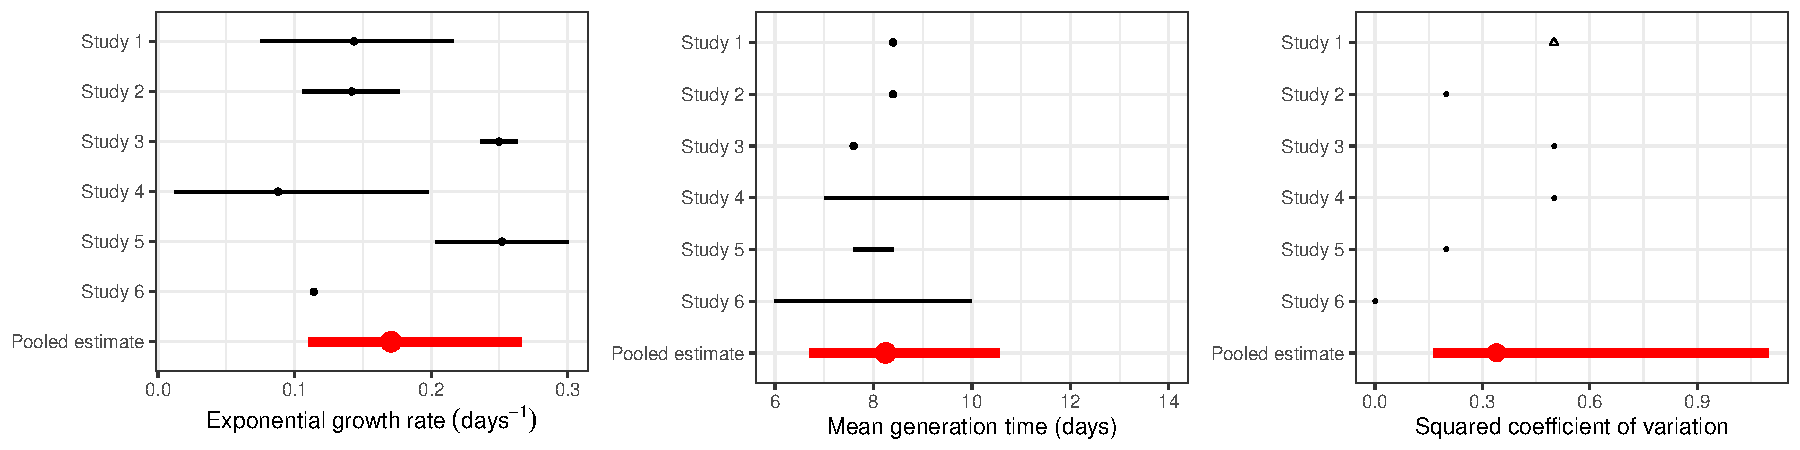
\includegraphics[width=\textwidth]{compare_assumption.pdf}
\caption{
\textbf{Comparisons of the reported parameter values with our pooled estimates.}
We inferred point estimates (black), uniform distributions (orange) or confidence/credible intervals (purple) for each parameter from each study, and combined them into pooled estimates using a Bayesian multilevel model (red).
Points represent medians calculated from the parameter set $(\bar{G}_{i}, \kappa_{i}, r_{i})$ for each study $i$ (orange and purple).
Error bars represent 95\% equi-tailed quantiles calculated from the parameter set $(\bar{G}_{i}, \kappa_{i}, r_{i})$ for each study $i$.
Red violin plots represent distributions of 2000 posterior samples.
Open triangle: we assumed $\kappa=0.5$ for Study 2 which does not report generation-interval dispersion.
}
\label{fig:assumption}
\end{figure}

\fref{eff} shows how propagating uncertainty in different combinations would affect estimates and CIs for \Ro. 
For illustrative purposes, we use our pooled estimates, which may represent a reasonable proxy for the state of knowledge as of January 23--26, 2020 (\fref{eff}A).
Comparing the estimates that include only some sources of uncertainty to the pooled estimate ($\Rpool = 3.0$; 95\% CI: 2.1--4.6; see `all' in \fref{eff}), we see that propagating error from the growth rate (which all but one of the studies reviewed did) is absolutely crucial: two middle bars ($\mu_G$ and $\mu_\kappa$), which lack growth-rate uncertainty, is relatively narrow.
In this case, propagating error from the mean generation interval has negligible effect compared to propagating the uncertainty in $r$.
Uncertainty in the generation-interval dispersion $\kappa$ also has important effects as it determines the functional form of the relationship between $r$ and \Ro (compare $\mu_G$ with $\mu_\kappa$).
For example, reducing $\kappa$ from 1 (assuming exponentially distributed generation intervals) to 0 (assuming fixed generation intervals) changes the $r$--\Ro\ relationship from linear to exponential (see \eref{gamma}), therefore increasing the sensitivity of \Ro estimates to $r$ and $\bar G$.
We note that our estimate of \Rpool is relatively insensitive to our assumption of $\kappa=0.5$ for Study 2: assuming $\kappa=0.1$ gives $\Rpool = 3.0$ (95\% CI: 2.2--4.7), whereas assuming $\kappa=0.9$ gives $\Rpool = 2.9$ (95\% CI: 2.1--4.4).

We further explore how the effects of uncertainties in generation-interval distributions change when there is less uncertainty associated with the exponential growth rate.
This hypothetical example reflects recent scenarios, as increased data availability will allow researchers to estimate $r$ with more certainty.
To simulate estimates of the exponential growth rate with stronger confidence, we use $\hat{\mu}_r = (\mu_r + 3\times\mathrm{median}(\mu_r))/4$ instead of $\mu_r$ (\fref{eff}B); 
then $\hat{\mu}_r$ has the same median as $\mu_r$ but the associated 95\% CI is 4 times narrower (0.16--0.19 $\textrm{days}^{-1}$).
As uncertainty associated with the exponential growth rate decreases, accounting for uncertainties in generation intervals becomes even more important.
Propagating error only from the growth rate gives very narrow credible intervals in this case. 
Propagating errors from the mean generation interval or generation-interval dispersion gives wider but still narrow credible intervals.

\begin{figure}[!ht]
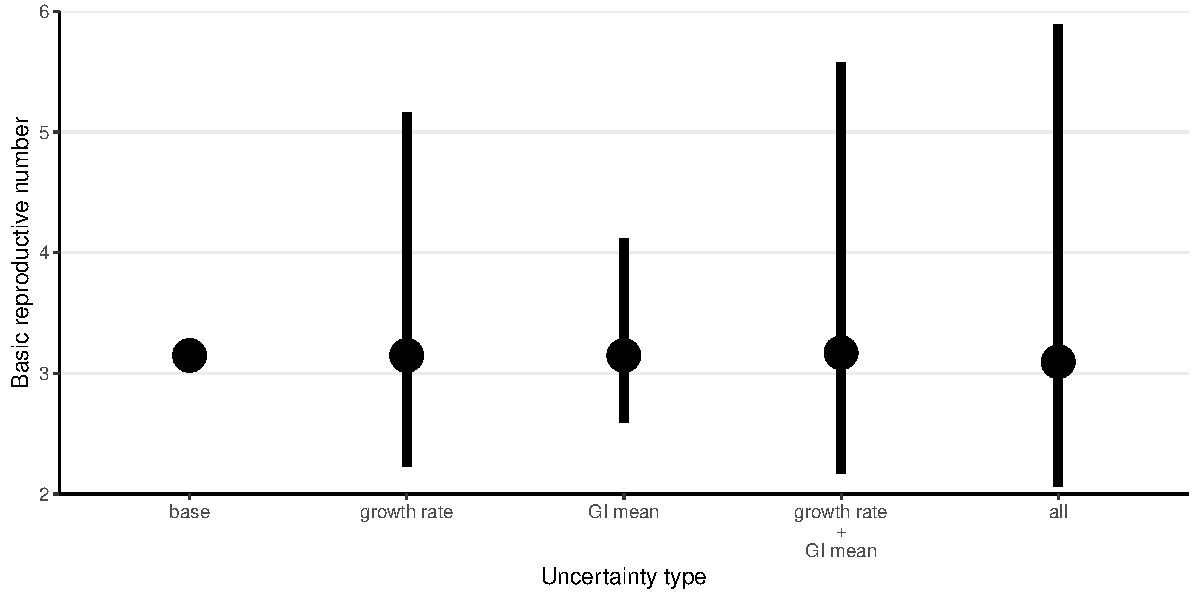
\includegraphics[width=\textwidth]{figure2.pdf}
\caption{
  \textbf{Effects of $r$, $\bar G$, and $\kappa$ on the estimates of \Ro.}
We compare estimates of \Ro under five scenarios that propagate different parameter uncertainties (A) based on our pooled estimates ($\mu_r$, $\mu_G$, and $\mu_\kappa$) and (B) assuming a 4-fold reduction in uncertainty of our pooled estimate of the exponential growth rate (using $\hat{\mu}_r = (\mu_r + 3\times\mathrm{median}(\mu_r))/4$ instead of $\mu_r$).
Each uncertainty type represents \Ro estimates based the posterior distributions of one of three parameters ($\mu_r$, $\mu_G$, and $\mu_\kappa$) while using median estimates of two other parameters.
The `base' type represents \Ro estimate based on the median estimates of $\mu_r$, $\mu_G$, and $\mu_\kappa$.
The `all' type represents \Ro estimates based on the joint posterior distributions of  $\mu_r$, $\mu_G$, and $\mu_\kappa$.
Points represent the median estimates.
Vertical error bars represent the 95\% credible intervals.
}
\label{fig:eff}
\end{figure}

Finally, \fref{R0} compares the ``base'' estimates (based on $r_i$, $\bar G_i$, and $\kappa_i$ for each study $i$) and 21 substitute estimates (3 parameter substitutions $\times$ 7 studies).
All but 8 substitute estimates have wider credible intervals compared to their corresponding base estimates --- namely, $\bar G$-substitute estimates for Study 1 and 7, $r$-substitute estimates for Study 1 and 2, and  $\kappa$-substitute estimates for Study 3, 6, and 7.
Furthermore, accounting for uncertainties in the estimate of $r$ has the largest effect on the estimates of \Ro\ in most cases (\fref{R0}).
For example, the $r$-substitute estimate of \Ro for Study 7 is $\Ro = 3.9$ (95\% CI: 2.3--8.8), which is much wider than the uncertainty range they reported (2.0--3.1).
This is consistent with our earlier results (\fref{eff}) that demonstrated the importance of accounting for uncertainty in the exponential growth rate $r$.
We also note that the pooled estimate of the basic reproduction number ($\Rpool = 3.0$; 95\% CI: 2.1--4.6) has wider credible intervals than the base estimates except for Study 2.


\begin{figure}[!th]
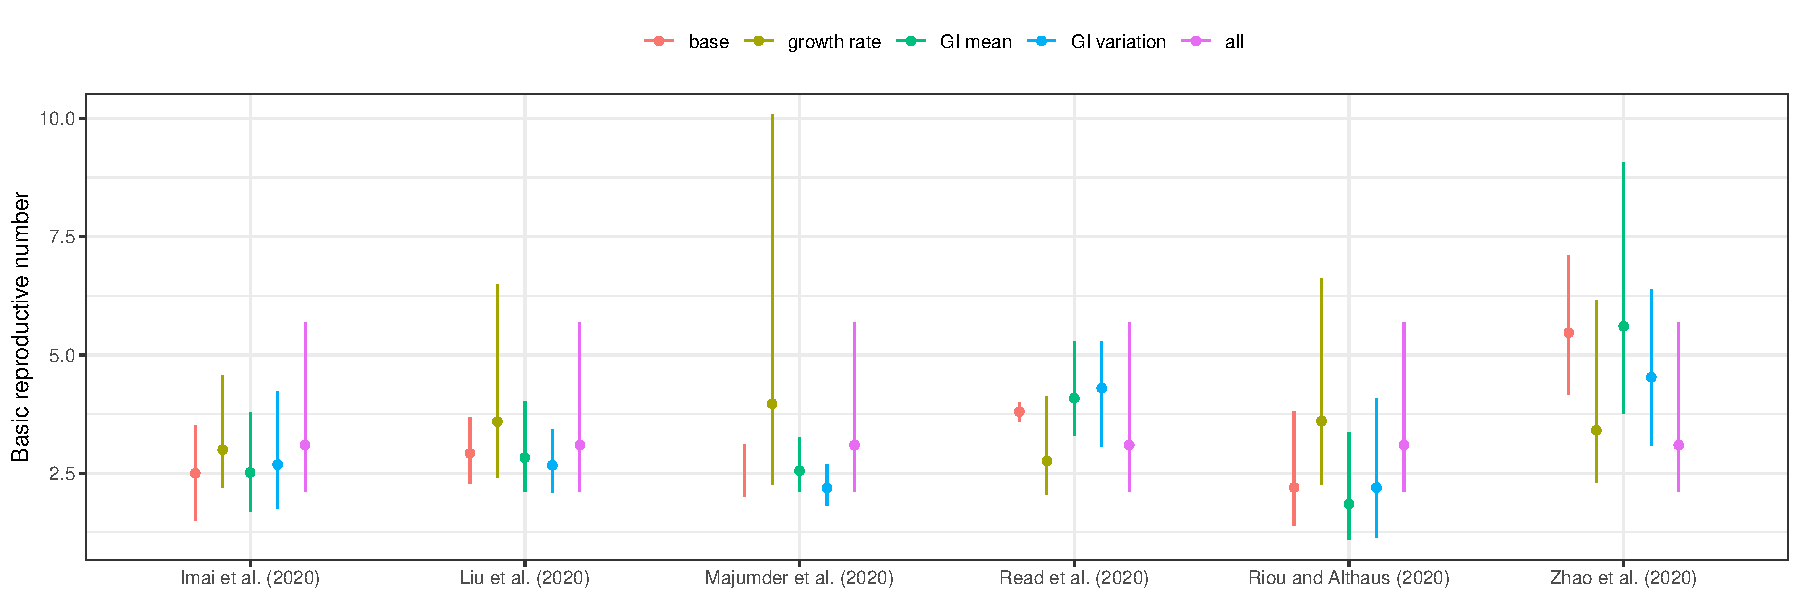
\includegraphics[width=\textwidth]{compare_R0.pdf}
\caption{
\textbf{Sensitivity of the reported \Ro estimates with respect to our pooled estimates of the underlying parameters.}
We replace the reported parameter values (growth rate $r$, mean generation interval $\bar G$, and generation-interval dispersion $\kappa$) with our corresponding pooled estimates ($\mu_r$, $\mu_G$, and $\mu_\kappa$) one at a time and recalculate \Ro (\textbf{growth rate}, \textbf{mean generation interval}, and \textbf{generation-interval dispersion}).
The pooled estimate of \Ro is calculated from the joint posterior distribution of $\mu_r$, $\mu_G$, and $\mu_\kappa$ (\textbf{all});
this corresponds to replacing all reported parameter values with our pooled estimates, which gives identical results across all studies.
Horizontal dashed lines represent the 95\% credible intervals of our pooled estimate of \Ro.
The reported \Ro estimates (\textbf{base}) have been adjusted to show the approximate 95\% credible interval using the probability distributions that we defined if they had relied on different measures for parameter uncertainties.
}
\label{fig:R0}
\end{figure}

\section{Discussion}

Estimating the basic reproductive number \Ro is crucial for predicting the course of an outbreak and planning intervention strategies.
Here, we use a gamma approximation \citep{park2019practical} to decompose \Ro estimates into three key quantities ($r$, $\bar G$, and $\kappa$) and apply a multilevel Bayesian framework to compare estimates of \Ro for the SARS-CoV-2 outbreak.
Our results demonstrate the importance of accounting for uncertainties associated with the underlying generation-interval distributions, including uncertainties in the amount of dispersion in the generation intervals.

Our analysis shows that many early estimates of \Ro rely on strong assumptions.
The lack of uncertainties in the generation-interval dispersion is particularly surprising because it determines the shape of the $r$-\Ro relationship (\fref{assumption});
assuming fixed parameter values can lead to overly strong conclusions \citep{elderd2006uncertainty}.
The lack of uncertainties in the generation-interval dispersion further explains the sensitivity of \Ro estimates to the exponential growth rate, particularly in Study 7 (\fref{R0}).
Since Study 7 assumes a fixed generation interval ($\kappa=0$), they implicitly assume an exponential $r$--\Ro relationship, making their estimate too sensitive to $r$.
One exception is Study 1: we find this estimate of \Ro is most sensitive to generation-interval dispersion $\kappa$.
This is because Study 1 assumes an exponentially distributed generation interval ($\kappa=1$): estimates that rely on this assumption make \Ro relatively insensitive --- implicitly assuming a linear $r$--\Ro relationship --- and thus tend to have particularly narrow credible intervals.

As most studies rely on strong assumptions, the credible intervals associated with the base \Ro estimates are necessarily narrower than the credible intervals of the pooled estimate ($\Rpool = 3.0$; 95\% CI: 2.1--4.6).
While the point estimate of \Rpool is similar to other reported values from this date range, the credible intervals are wider than all but one study.
This result does not imply that assumptions based on the pooled estimate are too weak;
we believe that this credible interval more accurately reflects the level of uncertainties present in the information that was available when these models were fitted.
In fact, because the pooled estimate does not account for overlap in data sources used by the models, we feel that it is more likely to be over-confident than under-confident.
Our median estimate averages over the various studies, and therefore particular studies have higher or lower median estimates.
We note in particular that, while the baseline example we used from Study 6 may appear to be an outlier, the authors of this study also explore different scenarios involving changes in reporting rate over time, under which their estimates of \Ro are similar to other reported estimates.
Here, our focus is on estimating uncertainty, not on identifying potential explanations for these discrepancies.

Of the seven studies that we reviewed, two of them directly fit their models to cumulative number of confirmed cases.
This approach can be appealing because of its simplicity and apparent robustness, but fitting a model to cumulative incidence instead of raw incidence can both bias parameters and give overly narrow confidence intervals, if the resulting non-independent error structures are not taken into account \citep{ma2014estimating, king2015avoidable}.
Narrow uncertainties in the estimates of the exponential growth rate are likely to depend on this assumption.
Naive fits to cumulative incidence data should therefore be avoided.

Many sources of noise affect real-world incidence data, including both dynamical, or ``process'', noise (randomness that directly or indirectly affects disease transmission); and observation noise (randomness underlying how many of the true cases are reported).  
Disease modelers face the choice of incorporating one or both of these in their data-fitting and modeling steps. 
This is not always a serious problem, particularly if the goal is inferring parameters rather than directly making forecasts \citep{ma2014estimating}.
Modelers should however be aware of the possibility that ignoring one kind of error can give overly narrow confidence intervals \citep{king2015avoidable,taylor2016stochasticity}.

There are other important phenomena not covered by our simple framework.
Examples that seem relevant to this outbreak include: changing reporting rates, reporting delays (including the effects of weekends and holidays), and changing generation intervals.
For emerging pathogens such as SARS-CoV-2, there may be an early period of time when the reporting rate is very low due to limited awareness or diagnostic resources;
for example, \cite{zhaoncov} (Study 6) demonstrated that estimates of \Ro can change from 5.47 (95\% CI: 4.16--7.10) to 3.30 (95\% CI: 2.73--3.96) when they assume 2-fold changes in the reporting rate between January 17, when the official diagnostic guidelines were released \citep{who17protocol}, and January 20.
Delays between key epidemiological timings (e.g., infection, symptom onset, and detection) can also shift the shape of an observed epidemic curve and, therefore, affect parameter estimates as well as predictions of the course of an outbreak \citep{tariq2019assessing}.
Even though a constant delay between infection and detection may not affect the estimate of the growth rate, it can still affect the associated credible intervals.
Other factors related to reporting --- including changes in case definition, saturation in diagnostic test capacity, transparency of data, and representativeness of samples --- will also affect the inference.
Finally, generation intervals can become shorter throughout an epidemic as intervention strategies, such as quarantine, can reduce the infectious period \citep{hethcote2002effects};
since we are primarily focusing on the outbreak in Wuhan city before confinement, generation intervals are unlikely to vary significantly.
All of these factors affect the estimation of the exponential growth rate, which, in turn, will affect the estimation of the basic reproduction number.

Here, we focused on the estimates of \Ro that were published within a very short time frame (January 23--26, 2020).
Since the estimates were published as pre-prints, rather than in peer-reviewed journals, the quality of the analyses as well as the resulting estimates have not been finalized.
For example, Study 4 initially estimated $\Ro = 3.8$ (95\% CI: 3.6--4.0; \cite{readncov}) but revised their estimate on January 28, 2020: $\Ro = 3.11$ (95\% CI: 2.39--4.13; \cite{readncov2});
we did not include their revised estimates in our analysis in order to focus on available information at the very beginning of the outbreak.
Some studies also do not provide detailed description of their methods, data, and/or assumptions.
The quality of these analyses adds further uncertainty to their results that are not captured by their uncertainty quantification (e.g., reported credible intervals) or by our analysis.
While pre-prints can play an important role in disseminating information, they should be interpreted with care.

During early phases of an outbreak, it is reasonable to assume that the epidemic grows exponentially \citep{anderson1991infectious}.
However, as the number of susceptible individuals decreases, the epidemic will saturate, and estimates of $r$ used for \Ro should account for the possibility that $r$ is decreasing through time.
Although our analysis only reflects a snapshot of a fast-moving epidemic, we expect certain lessons to hold: credible intervals must combine different sources of uncertainty. 
In fact, as epidemics progress and more data becomes available, it is likely that inferences about exponential growth rate (and other epidemiological parameters) will become more precise; thus the risk of over-confidence when uncertainty about the generation-interval distribution is neglected will become greater.

We strongly emphasize the value of attention to accurate characterization of the transmission chains via contact tracing and better statistical frameworks for inferring generation-interval distributions from such data \citep{britton2019estimation}.
A combined effort between public-health workers and modelers in this direction will be crucial for predicting the course of an epidemic and controlling it.
We also emphasize the value of transparency from modelers.
Model estimates during an outbreak, even in pre-prints, should include code links and complete explanations.
We suggest using methods based on open-source tools allow for maximal reproducibility.

\cite{flaxman2020estimating} recently estimated the basic reproduction number for SARS-CoV-2 outbreaks in 11 European countries to be around 3.87 (3.01--4.66), on average.
While these estimates appear to be broadly consistent with to earlier estimates from China, comparing the exponential growth rate and the underlying generation-interval distributions suggest otherwise.
They assumed a shorter mean generation interval ($\bar G = 6.5\,\textrm{days}$) but similar generation-interval dispersion ($\kappa = 0.38$);
based on these values, the exponential growth rate has to be much higher ($r = 0.27\,\textrm{days}^{-1}$) to obtain $\Ro = 3.87$ compared to the exponential growth rate observed in China ($\mu_r = 0.17\,\textrm{days}^{-1}$; 95\% CI: 0.12--0.25 $\textrm{days}^{-1}$).
We caution that naively comparing estimates of the basic reproduction number without accounting for differences in underlying assumptions can underestimate the differences in the estimates.

In summary, we have provided a basis for comparing exponential-growth based estimates of \Ro and its associated uncertainty in terms of three components: the exponential growth rate, mean generation interval, and generation interval dispersion. 
We hope this framework will help researchers understand and reconcile disparate estimates of disease transmission early in an epidemic.

\pagebreak

\section*{Funding}

BMB and DJDE were supported by Natural Sciences and Engineering Research Council (NSERC). ML was supported by Canadian Institutes of Health Research (CIHR). The funders had no role in study design, data collection and analysis, decision to publish, or preparation of the manuscript.

\section*{Competing interests}

We declare no competing interests.

\section*{Acknowledgements}

We thank Daihai He for providing helpful comments on the manuscript.

\section*{Contribution}

SWP and JD developed the statistical framework. 
SWP reviewed the published literature.
SWP performed the analysis. 
SWP, BMB, and JD created the figures. 
SWP and JD wrote the first draft.
All authors contributed to the writing and approval of the final report.

\section*{Data availability}

\texttt{R} code is available in GitHub (\url{https://github.com/parksw3/nCoV_framework}).


\pagebreak

\bibliography{ncov_abbr}

\pagebreak
\appendix
\renewcommand\thefigure{A\arabic{figure}}
\setcounter{figure}{0}    
\section*{Appendix}

\begin{figure}[!h]
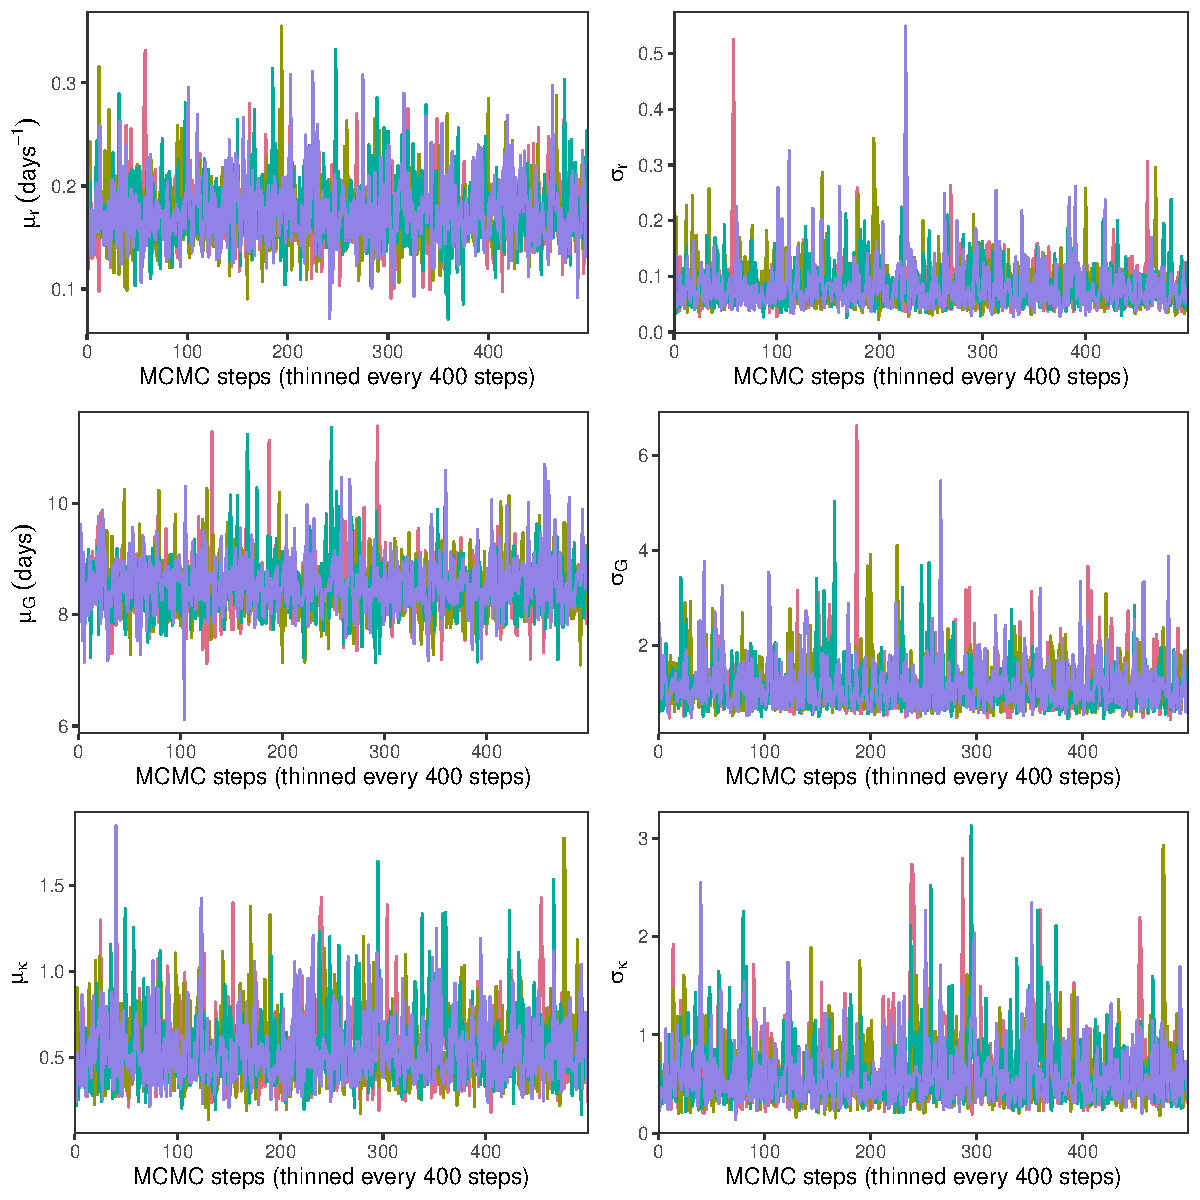
\includegraphics[width=\textwidth]{posterior_chain.pdf}
\caption{
\textbf{Trace plots of the multilevel model.}
Each chain is represented by a different color.
}
\end{figure}

\pagebreak

\begin{figure}[!h]
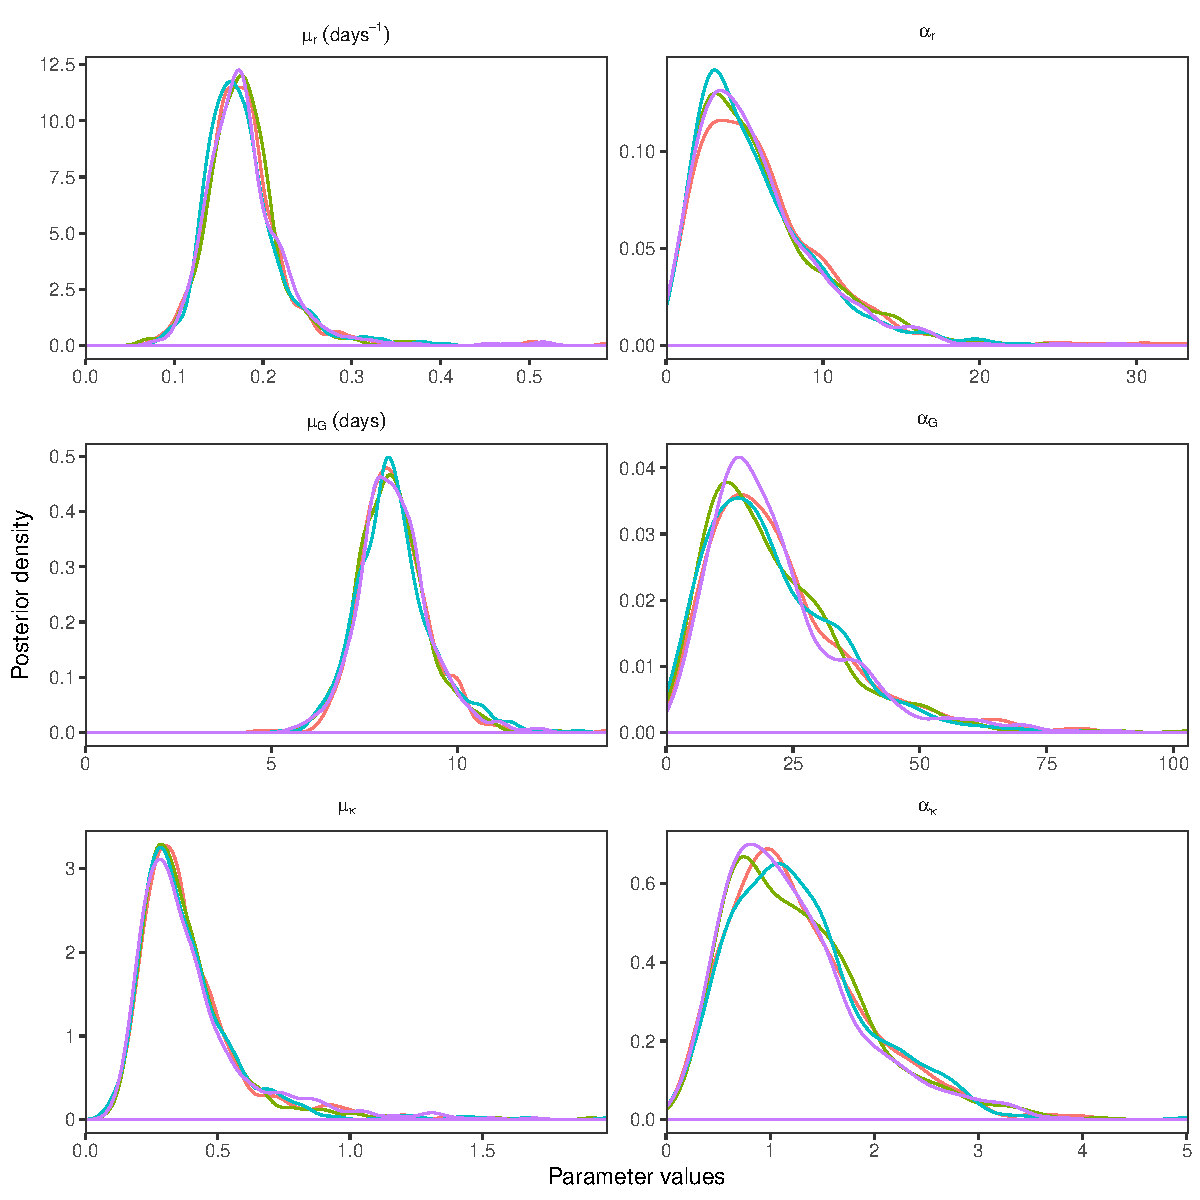
\includegraphics[width=\textwidth]{posterior_dist.pdf}
\caption{
\textbf{Marginal posterior distributions of the multilevel model.}
Each chain is represented by a different color.
}
\end{figure}

\end{document}
